\subsection{Selection optimization}
\label{sec:enujjOptimization}    

The final event selection criteria are optimized by maximizing the expected signal significance defined as 
$S/\sqrt{S+B}$, where S (B) is the expected number of signal (background) events passing the 
selection requirements. An additional requirement of \mt$>120$ GeV is imposed to remove background events with on-shell Ws. 
Then, three variables (\st,~\MET, and~\mej) are optimized 
simultaneously by scanning appropriate ranges of values.
Figure \ref{fig:enujj-optimization} shows the smooth dependence of the 
optimized \mej~and \st~cut values on the leptoquark mass hypothesis.
\begin{figure}
  \begin{center}
    {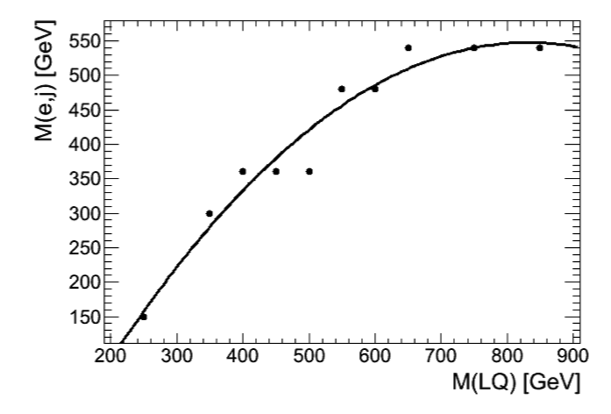
\includegraphics[width=.45\textwidth]{tex/analysis/event_selection/fig/optimization/optimization_enujj_mej.png}}
    {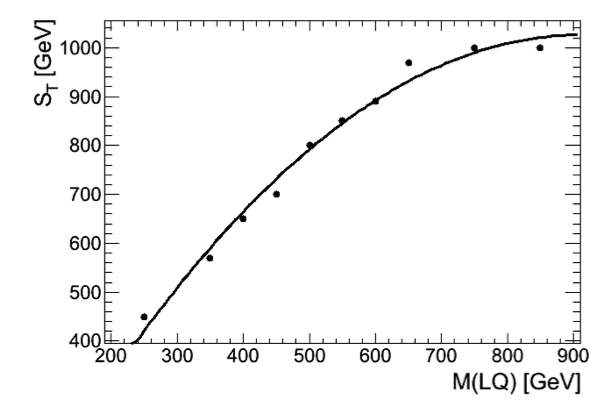
\includegraphics[width=.45\textwidth]{tex/analysis/event_selection/fig/optimization/optimization_enujj_st.png}}
    \caption{
      Optimized thresholds for for \mej~(left) and \st~(right) cuts
      as a function of leptoquark mass in the \enujj~channel.
      The leptoquark mass hypothesis under consideration is shown on the $x$-axis.
      The optimized cut thresholds are shown on the $y$-axis.
      The resulting distributions are fit with a second-degree polynomial.
    }
    \label{fig:enujj-optimization}
  \end{center}
\end{figure}
The results of the optimization, obtained for each LQ mass hypothesis, 
are summarized in Table~\ref{tab:enujjOptimizedCuts} assuming an 
integrated luminosity of \lumi.
\begin{table}
  \centering
  \begin{tabular}{l | c | c | c | c | c | c | c | c | c | c } 
    \MLQ~[GeV]  & 250 & 350 & 400 & 450 & 500 & 550 & 600 & 650 & 750 & 850 \\ 
    \hline 
    \hline 
    \st~[GeV]  & 450 & 570 & 650 & 700 & 800 & 850 & 890 & 970 & 1000 & 1000 \\ 
    \hline 
    \MET~[GeV]  & 100 & 120 & 120 & 140 & 160 & 160 & 180 & 180 & 220 & 240 \\ 
    \hline 
    \mej~[GeV]  & 150 & 300 & 360 & 360 & 360 & 480 & 480 & 540 & 540 & 540 \\ 
  \end{tabular}
  \caption{Optimized selection criteria for the \enujj analysis for different LQ mass hypotheses. 
    The requirement \mt$>120$~\GeV is applied to all mass hypotheses.
  }
  \label{tab:enujjOptimizedCuts}
\end{table}

